\documentclass{article}

% preamble.tex source: Templates for CCSC Conferences (paper_template)
% https://github.com/ccsc-journal/ccsc-editor/tree/master
\input{preamble}

\addbibresource{paper.bib}

%path to figures - \usepackage{graphicx} is included in preamble.tex
\graphicspath{{figures/}}

\title{Hierarchical Web of Hypernetwork Experts for mitigating catastrophic forgetting in Audio Classification\footnote{CSCI 693 Research Methods in Computer Science, Spring 2026}}

\author{
  Alexander Baron, Shelley Wong\\
  Computer Science Department\\
  California State University, Chico\\
  Chico, CA 95929\\
  \email{\{ajbaron,swong26\}@csuchico.edu}
}

\begin{document}
\maketitle

\begin{center}
    \begin{minipage}{0.7\textwidth}
        \begin{center}
            \begin{large}
                \textbf{Abstract}\\
            \end{large}
        \end{center}
Modern neural networks often favor monolithic architectures, where global weight updates for new tasks often overwrite critical feature mappings, a failure mode known as Catastrophic Forgetting. This paper introduces a Hierarchical Web of Hypernetwork Experts, a modular framework that departs from the monolithic paradigm by utilizing a Directed Acyclic Graph of specialized neural Nodes. Unlike standard approaches that update a single global parameter space, our architecture employs a hypernetwork driven routing logic to isolate learning, ensuring that new knowledge acquisition does not degrade previously mastered feature sets. We evaluate this approach on the multi-label MagnaTagATune dataset. The proposed architecture achieved a 37\% micro-F1 score, performing competitively with monolithic baselines while demonstrating superior structural plasticity, and knowledge retention during iterative expansion.
    \end{minipage}
\end{center}
\\\
\section{Introduction}
Deep neural networks exhibit a well-documented failure mode known as catastrophic forgetting, where the acquisition of new task knowledge causes severe degradation of previously learned representations. This research addresses this limitation within the MagnaTagATune benchmark, a challenging multi-label audio classification task that requires the identification of 188 distinct tags in~25,000 audio segments, curated by \textcite{MagnaTag}. Unlike standard monolithic architectures that utilize a single global parameter space, our approach utilizes a Hierarchical Web of Hypernetwork Experts. This framework departs from the status quo by employing a Directed Acyclic Graph (DAG) where nodes function as specialized modules. By isolating updates to specific experts via a hypernetwork driven routing logic, we preserve modular knowledge and mitigate weight overwriting.

\subsection{Definition of Terms}
\begin{itemize}
    \item \textbf{Audio Source Processing}: A broad category of signal processing tasks concerned with the analysis of individual audio sources, encompassing both the classification of source types and the separation of mixed audio signals into their constituent components.
    \item \textbf{Multi-Label Audio Classifier}: A neural network model that produces multiple simultaneous predictions for a single audio input. In contrast to single-label classifiers, which assign exactly one category per input.
    \item \textbf{Mixture-of-Experts (MoE)}: A neural network architecture consisting of a set of specialized sub-networks, referred to as experts, governed by a learned gating mechanism. The gating mechanism dynamically selects or weights a subset of experts for each input, enabling the model to partition its capacity across distinct functional regions of the input space.
    \item \textbf{Graph}: A mathematical structure used to represent relational data, consisting of a set of entities (nodes) and the pairwise relationships between them (edges). Graphs provide a flexible representation for data whose structure cannot be adequately captured by standard Euclidean formats such as grids or sequences.
    \item \textbf{Nodes}:  The fundamental unit of a graph, representing an individual data entity. Nodes may carry associated feature vectors and are connected to other nodes via edges.
    \item \textbf{Edges}:  A structural element of a graph encoding a relationship between two nodes. Edges may be undirected, indicating a symmetric relationship between the connected nodes, or directed, indicating an asymmetric relationship in which one node influences or references another.
    \item \textbf{Graph Neural Network (GNN)}: A class of neural networks designed to operate directly on graph-structured data. GNNs learn node and edge representations by iteratively aggregating and transforming feature information across local neighborhoods, enabling the model to capture both local structure and global context.
    \item \textbf{Hyper Networks}: A neural network that generates the weight parameters of a separate, typically larger target network. Rather than learning fixed weights directly, the hypernetwork conditions weight generation on some input context, enabling dynamic and parameter-efficient adaptation of the target network.
    \item \textbf{Genetic Algorithms}: A class of optimization algorithms inspired by biological evolution. Over successive generations, a population of candidate solutions undergoes selection, mutation, and recombination. Operations may also include pruning connections, freezing parameters, or introducing new nodes and edges guided by a fitness function that evaluates solution quality.
    \item \textbf{Neuroevolution of Augmenting Topologies (NEAT)}:  A genetic algorithm specifically designed for the evolution of neural network architectures. NEAT simultaneously optimizes both the weight parameters and the structural topology of networks, allowing complexity to grow incrementally through the addition of nodes and connections over successive generations.
\end{itemize}

\section{Related Work}

\subsection{Waveform vs. Spectrograms}
Audio source processing relies on one of two primary signal representations: spectrograms or raw waveforms. A spectrogram is a time-frequency representation that encodes perceptually meaningful acoustic structure by mapping a signal’s energy distribution across both time and frequency. Raw waveforms, by contrast, represent amplitude as a function of time and preserve information that spectrograms inherently discard, including phase, fine-grained temporal structure, and transients.
Spectrograms have dominated audio machine learning research in recent years, owing to their computational efficiency and interpretability. However, the spectrogram pipeline introduces irreversible information loss; phase is typically discarded during transformation, and transient details may be smoothed or aliased depending on the window parameters used. Waveform-based models avoid this loss entirely, preserving the full fidelity of the original signal. This completeness comes at a cost; raw waveforms are higher dimensions, lack the structured frequency that convolutional architectures exploit in spectrograms, and generally impose greater computation demands during training and inference.\\

\noindent Despite these challenges, the representation completeness and architectural flexibility of waveform-based approaches have driven renewed interest in the paradigm, with models such as WaveNet, SampleCNN, and EnCodec demonstrating competitive or superior performance across a range of audio tasks. The present research adopts a waveform-based representation exclusively, motivated by the preservation of phase and temporal information that are potentially relevant to fine-grained multi-label classification.

\subsection{Mixture-of-Experts}
The Mixture-of-Experts framework was introduced by \textcite{Jacobs1991} and further formalized by \textcite{HMoE_Em}, who proposed partitioning the input spaces among a set of specialized sub-networks, referred to as experts, governed by a learn routing function. The central premise of the architecture is that not all parameters need to be active for every input.\\

\noindent \textcite{Outrageous} extended this framework to large-scale sequence modeling by introducing a sparsely gated MoE layer interleaved between Long Short-Term Memory (LSTM) layers, in which only the top-k experts are activated per token. While this approach demonstrated substantial gains in model capacity without proportional increases in computational cost, it also exposed a critical instability: in the absence of explicit load-balancing regularization, routing functions tend to collapse, concentrating activation onto a small subset of experts and leaving the remainder undertrained.\\

\noindent The present research adopts the core MoE principle of input-space partitioning among specialized sub-networks, adapting it to the continual learning setting where expert modules must be incrementally generated and integrated without disrupting previously acquired representation.

\subsection{Continual Learning}
Continual learning, also referred to as lifelong learning or incremental learning, addresses the problem of training a model sequentially across a series of tasks while retaining previously acquired knowledge. The central failure mode of this paradigm was identified by \textcite{CatastrophicI}, who characterized catastrophic forgetting as the tendency of neural networks to overwrite weight configurations that encode prior task representations when updated on new data. This interference arises from the distributed nature of gradient-based learning: because knowledge is encoded diffusely across shared parameters, updates targeted at a new task inevitably degrade performance on earlier ones. The present research situates itself within this framework by targeting catastrophic forgetting specifically in the context of multi-label audio classification, where the task distribution is non-stationary. 

\subsection{Hyper Networks}
The hypernetwork framework was introduced by \textcite{Hypernetworks}, who proposed using a small auxiliary network to generate the weight parameters of a separate, larger target network. Rather than directly optimizing the target network’s weights through gradient descent, the hypernetwork learns a compressed mapping from an embedding space to a target network’s weight space, enabling a form of relaxed weight-sharing across layers. \textcite{Hypernetworks}. demonstrated this approach across both convolutional and recurrent architectures, achieving competitive performance on sequence modeling tasks while requiring fewer learnable parameters than conventionally trained networks.\\

\noindent \textcite{ContinualLearningHyper} extended this framework to the continual learning setting by introducing task-condition hypernetworks, in which the hypernetwork receives a task-specific embedding as input and generates the full weight configuration of a target model for that task. This design sidesteps catastrophic forgetting by decoupling task-specific weight realizations from one another, rather than overwriting shared parameters. Each new task is encoded as a distinct embedding that produces its own weight instantiation. Previous task knowledge is preserved through a lightweight output regularizer that constrains the hypernetwork’s outputs on prior task embeddings to remain stable during new task training. \\

\noindent The present research builds directly on this line of work by employing a hypernetwork to generate the weights of newly instantiated expert modules within the MoE framework. Rather than conditioning weight generation on a global task identity, the hypernetwork here operates at the expert level, producing specialized parameter configurations for each new classification as it is introduced into the system.\\

\subsection{Synthesis}
The present research converges the four domains into a novel architecture designed for scalable, multi-label audio classification. Our architectures adopts raw waveform processing, through the implementation of ReSEBlocks (Residual Squeeze-and-Excitation). By operating directly on the temporal domain, the model preserves the phase and transient fidelity necessary to distinguish subtle instrument textures in the MagnaTagATune dataset. \\

\noindent To manage the high dimensionality of this data, we apply the Mixture-of-Experts principle, partitioning the input space into a Directed Acyclic Graph of AudioSpecialists. Unlike standard MoE layers that collapse into a few active parameters, our DAG structure forces a topological hierarchy, ensuring information flows through increasingly specialized modules. \\

\noindent To address catastrophic forgetting, we move away from monolithic weight updates that typically degrade prior knowledge. We integrate Hypernetworks not merely as parameter compressors, but as evolutionary engines. In our framework, the hypernetwork is responsible for generating the weight configuration of newly instantiated expert modules.\\

\noindent When the system detects stagnation, the Evolutionary Trainer will mutate the architecture, by adding a new specialist node with hypernetwork generated weights, stitching weight mappings via a partial identity copy mechanism, and adaptive gating, which employs sigmoid-based routing logic to isolate updates, ensuring new knowledge does not overwrite established representations

\section{Research Question & Hypothesis}

\subsection{Question}

Does NEAT-style topological discover network architectures that are better suited to continuous multi-label audio classification than fixed, predefined architectures, as measured by forward transfer, backward transfer, and overall classification performance across sequential tasks? Does the coupling strength between expert modules, as determined by the evolved graph structure, correlate with inter-task similarity, and if so, does this emergent specialization contribute to reduced catastrophic forgetting?\\\

\subsection{Hypothesis}

A hierarchical continual learning system in which NEAT-style topological evolution governs the structure of individual expert modules, and a graph neural network manages inter-expert communication across hierarchy levels, will demonstrate measurably lower rates of catastrophic forgetting and stronger forward transfer compared to fixed-architecture continual learning baselines of sequential label audio classification tasks.\\

\noindent The evolved expert modules are expected to develop more functional and functional internal representations than their fixed-architecture counterparts, due to the ability of NEAT to grow or prune connectivity in response to task-specific fitness pressure. GNN-mediated message passing will enable high-level coordination between experts, allowing the hierarchical controller to selectively recruit relevant expert knowledge without destructive interference to previously learned representations. Finally, the coupling strength between expert modules in the evolved graph structure will positively correlate with acoustic similarity between tasks, suggesting the system’s architecture itself encodes a form of implicit task-relatedness.

\section{Methodology}

\subsection{Baseline Model}
To establish a performance upper bound, we utilize a Monolithic ResNet-Baseline architecture. This model consists of a sequential stack of residual blocks with a depth-wise expansion of channels (32 -> 64 -> 128 -> 256 -> 512). It utilizes global average pooling and a static multi-label classification head. When trained on the full MagnaTagATune 188-tag vocabulary, this architecture achieves a 43\% Micro-F1 score.

The monolithic baseline serves as the architectural template for the individual experts, its primary component, the ReSEBlock shown in Listing 1 integrates residual learning with adaptive feature recalibration.

\begin{lstlisting}[language=Python,  caption= ReSEBlock]

class ReSEBlock(nn.Module):
	self.resblock = ResidualBlock(in_channels, 
                out_channels, kernel_size, pool_size)
	self.se = SqueezeExcite(out_channels)
\end{lstlisting}

\noindent The Residual Block shown in Listing 2 addresses the vanishing gradient problem by providing a shortcut connection (x + f(x)) via \textit{nn.Identity} or a 1 x 1 convolution. This helps maintain the high-frequency temporal transients that might otherwise be smoothed out across deep layers.

\begin{lstlisting}[language=Python,  caption= Residual Block]

class ResidualBlock(nn.Module):
	self.main = SimpleCNNBlock(in_channels, 
            out_channels, kernel_size, pool_size)
	self.residual = nn.Conv1d(in_channels, 
            out_channels, kernel_size = 1) if in_channels != 
            out_channels else nn.Identity()
\end{lstlisting}


\noindent The SqueezeExcite block in Listing 3 implements a form of self-attention on the channel dimension. The global average pooling compresses the temporal dimension into a channel descriptor which is the Squeeze side. Two linear Layers learn a non-linear mapping that produces a set of per-channel modulation weights. We initialized our reduction to 16, which is the main hyperparameter that balances the power of the SE block against computation overhead

\begin{lstlisting}[language=Python,  caption= Squeeze-and-Excitation Block]

class SqueezeExcite(nn.Module):
	self.fc1 = nn.Linear(channels, channels // reduction)
	self.fc2 = nn.Linear(channels // reduction, channels)
\end{lstlisting}


\subsection{Evolutionary GNN}
The proposed system deconstructs the traditional pipeline into a Hierarchical Web of Hypernetwork Experts. Each node in the graph is an AudioSpecialist module, preserving the fundamental unit of the baseline, the Residual Squeeze-and-Excitation Block.

\begin{table}[ht]
\caption{Structural Comparison}
\label{table:nonlin}
\centering
\footnotesize % Dropping to footnotesize helps on 5.5in paper
\begin{tabular}{lp{3.5cm}p{4cm}} % Manually setting widths
\toprule
\textbf{Component} & \textbf{Monolithic Baseline} & \textbf{Evolutionary GNN} \\ 
\midrule
Connectivity    & Static, Sequential            & Dynamic DAG, evolved via NEAT \\
Optimization    & Global gradient descent       & Hypernetwork generated weights \\
Channel Scaling & Predefined (32 $\to$ 512)     & Incremental, specialists added on-demand \\
Adaption        & Retraining required           & Weight stitching preserves mappings \\ 
\bottomrule
\end{tabular}
\end{table}

\noindent After the squeeze-and-excitation recalibration, the specialist performs an Adaptive Average Pooling to reduce the 1D temporal signal to a fixed-length vector, this vector is then stored in an \textit{activation\_history} buffer. This allows the Evolutionary Trainer to calculate cosine similarity between nodes. If two nodes develop nearly identical signatures, the system recognizes a function overlap and may apply pruning or coupling pressure to maintain diversity in the graph.\\

\noindent The transition from the static baseline to the dynamic web is managed by a Controller (Hypernetwork). Unlike the baseline, where weights are learned via standard backpropagation across a fixed path, the weights for new specialist nodes are generated on a task-specific context. When the EvolutionaryTrainer identifies a performance plateau, it triggers a mutation. This involves using the Hypernetworks to initialize a new specialist, and adding edges within the DAG to all the new expert to receive information from existing predecessor experts.\\

\noindent To Ensure the classification head can accommodate the new feature dimensions without losing the mapping already encoded in established experts, Dynamic Weight Stitching is applied.

\subsection{Experimental Protocol}
The model is trained on the MagnaTagATune dataset split into \textit{N} sequential tasks, where each tasks introduces a new subset of the 188-tag vocabulary. A mutation event is triggered when the validation micro-F1 stagnates for more than 10 epochs. Upon mutation, the EvolutionaryTrainer evaluates node fitness using eigenvector centrality, nodes below the 20th percentile are pruned, and a new Hypernetwork generated expert is introduced to capture the features of the current task


\section{Results and Discussion}
The results provide a nuanced view of structural evolution in audio classification. While the model achieved a peak Micro-F1 score of 37\% training the monolithic baseline of 43\%, this performance must be contextualized within the complexity of the label space. Unlike standard benchmarks that evaluate only the top 50 MagnaTagATune tags, reaching ~80\% F1, this research utilized the full 188-tag vocabulary. Given that State-of-the-Art (SOTA) performance often drops toward 60\% when according for the full distribution, a 37\% score for self evolving architecture represents a significant functional baseline.

\begin{figure}[ht]
  \centering
  \small % Keeps the font size consistent
  
  \begin{minipage}{0.48\textwidth}
    \centering
    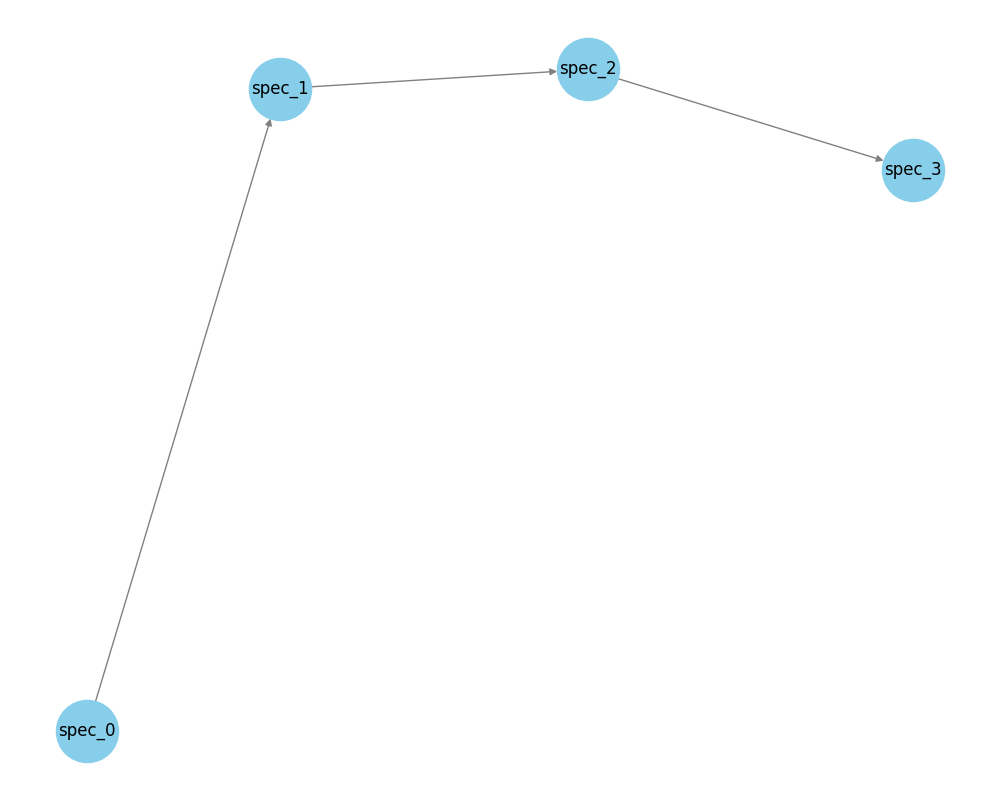
\includegraphics[width=\linewidth]{figures/plots/graph_epoch_9.png}
    \caption{Initial Graph}
    \label{fig:graph9}
  \end{minipage}
  \hfill % This adds space between the two images
  \begin{minipage}{0.48\textwidth}
    \centering
    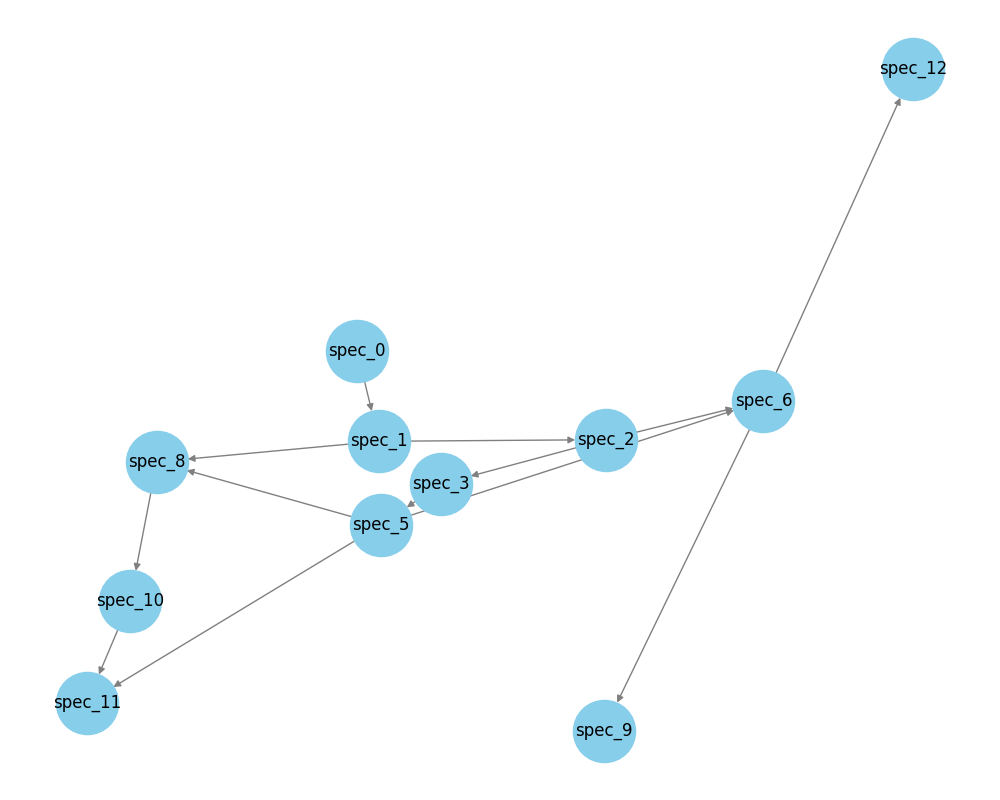
\includegraphics[width=\linewidth]{figures/plots/graph_epoch_259.png} % Replace with your 2nd file
    \caption{Graph after 250 epochs}
    \label{fig:graph10}
  \end{minipage}
\end{figure}\\\

\noindent Observations of the graphs evolution in Figure 1 and Figure 2 reveal a transition from a simple, nearly linear chain to a complex, interconnected Directed Acyclic Graph. By epoch 250, the network expanded from 4 initial nodes to 13 active specialists. This suggests the Evolutionary Trainer successfully identified performance plateaus, and introduce new parameters to capture residual variance. \\

\begin{figure}[ht]
    \large
    \centering
    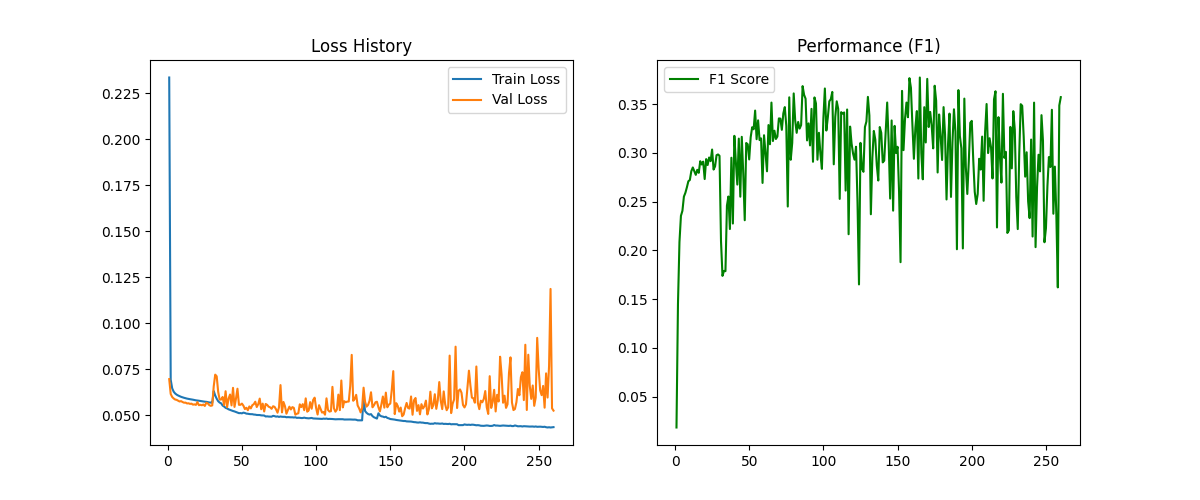
\includegraphics[width=\linewidth]{figures/plots/training_summary_epoch_260.png}
    \caption{Train Loss \& Validation Loss}
    \label{fig:epoch_sum260}
\end{figure}

\noindent The performance plot in Figure 3 shows significant volatility coinciding with mutation events. Specifically the sharp drops in F1 followed by rapid recovery mark the integration period where the system adapts to new branches. To prevent new, untrained modules from corrupting established feature mappings, parent weights were frozen during the first few epochs of a child node introducing. This allowed the architecture to converge the new modules into the existing knowledge base without destroying legacy representations. The integration of SE-gating proved critical for multi-expert communication. By providing a per-channel regularization, the gating mechanism allowed the model to prioritize relevant frequency channels and reduce noise interference between specialized nodes \\

\section{Conclusion}

While the peak Micro-F1 of 37\% sits below the monolithic baseline, the Hierarchical Web of Hypernetwork Experts demonstrates a clear advantage in structural stability and lifelong learning potential. Unlike traditional architectures that suffer from catastrophic forgetting or require complete retraining to accommodate new labels, this modular approach allows for incremental, non-destructive expansions.\\

\noindent To bridge this performance gap, I propose several critical refinements. The evolution cycle is currently highly sensitive to the cooling period. If the mutation interval is too aggressive, the architecture undergoes structural shifts before the weights can stabilize, effectively trapping the model in a sub-optimal saddle point within the loss landscape. Extending these convergence windows will allow for more robust parameter optimization between topological changes\\

\noindent Transitioning from random weight initialization to pre-trained specialist models could significantly accelerate the extraction of high level features. By priming roo nodes with weights from established audio benchmarks, the system would posses a more stable foundation for hierarchical growth. \\

\noindent Future iterations will explore Horizontal Expansion. While the current model primarily evolved in depth, increasing architectural width by introducing base nodes with vary channel capacities may allow the network to capture a more diverse array of acoustic signatures simultaneously \\

\noindent This project serves as a initial proof-of-concept for self-organizing machine learning systems. By shifting the paradigm from static, layer-based stacks to a dynamic, graph-based Web of Experts, we move closer to learning systems that do not merely process data, but actively adapt, specialize, and grow in complexity alongside the environments they inhabit
\\

\medskip

\printbibliography

\end{document}
